% ============================================================
% DIAGRAM: ResNet Residual Block (2015)
% ============================================================
% Caption: Figure 5.3: Residual block with identity shortcut.
%          (Adapted from He et al., 2015, p. 2)
% ============================================================

\documentclass[tikz,border=10pt]{standalone}
\usepackage{tikz}
\usepackage{amsmath}
\usepackage{amsfonts}

\usetikzlibrary{shapes,arrows,positioning,fit,calc,backgrounds}

\begin{document}

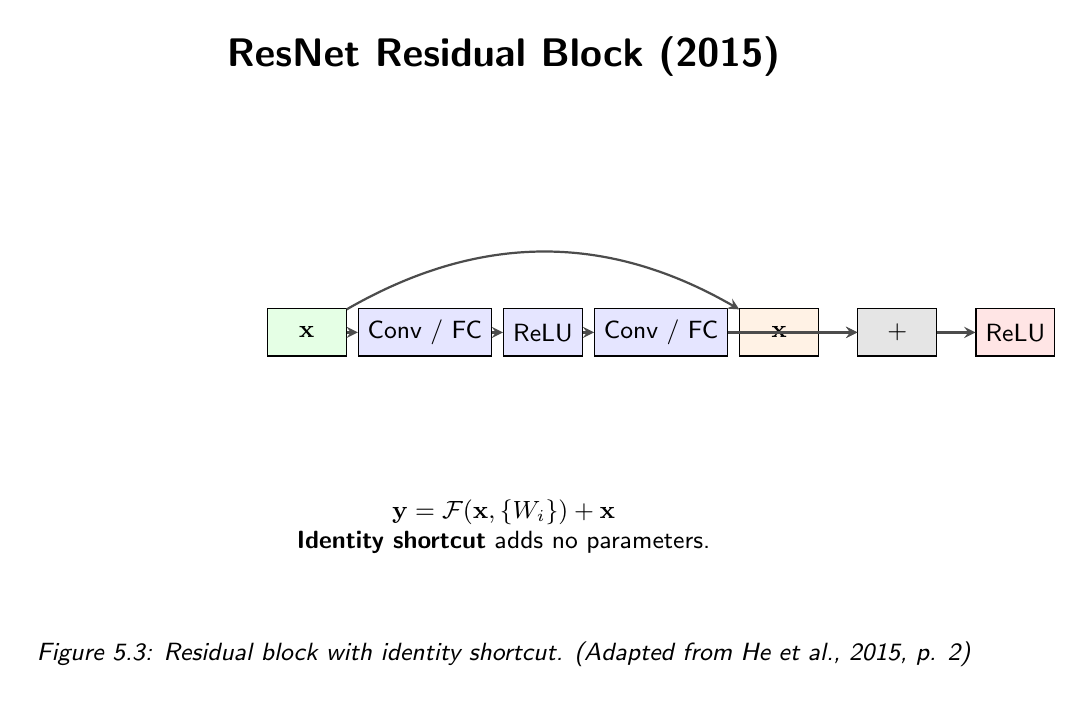
\begin{tikzpicture}[
    block/.style={draw, rectangle, minimum width=1cm, minimum height=0.6cm, fill=blue!10, font=\sffamily\small},
    edge/.style={-stealth, thick, draw=black!70},
    label/.style={font=\sffamily\small},
    title/.style={font=\sffamily\Large\bfseries},
    caption/.style={font=\sffamily\small\itshape},
]

\node[title] at (0, 3.5) {ResNet Residual Block (2015)};

% Input
\node[block, fill=green!10] (input) at (-2.5, 0) {$\mathbf{x}$};

% Weight layers
\node[block] (conv1) at (-1, 0) {Conv / FC};
\node[block] (relu) at (0.5, 0) {ReLU};
\node[block] (conv2) at (2, 0) {Conv / FC};

% Identity shortcut
\node[block, fill=orange!10] (shortcut) at (3.5, 0) {$\mathbf{x}$};

% Sum
\node[block, fill=gray!20] (add) at (5, 0) {$+$};

% Output
\node[block, fill=red!10] (out) at (6.5, 0) {ReLU};

\draw[edge] (input) -- (conv1);
\draw[edge] (conv1) -- (relu);
\draw[edge] (relu) -- (conv2);
\draw[edge] (conv2) -- (add);
\draw[edge] (shortcut) -- (add);
\draw[edge] (add) -- (out);

% Identity shortcut curve
\draw[edge, bend left=30] (input) to (shortcut);

% Equation
\node[align=center, font=\sffamily\small, anchor=north] at (0, -2.0) {
  $\mathbf{y} = \mathcal{F}(\mathbf{x}, \{W_i\}) + \mathbf{x}$ \\
  \textbf{Identity shortcut} adds no parameters.
};

\node[caption, anchor=north] at (0, -3.8) {
  Figure 5.3: Residual block with identity shortcut. (Adapted from He et al., 2015, p. 2)
};

\end{tikzpicture}
\end{document}
